\subsection{A Model for DevOps Adoption and Its Application}\label{sec:case_study}

Based on H1-H4 hypothesis, we present a three step model that
explains how to adopt DevOps according to our understanding. The
model considers the following steps:

\begin{enumerate}
\item In the first step, a company should
disseminate that the goal with a DevOps adoption is to
establish a \cc between
development and operations teams.

\item In the second step, a company should select and develop
the most suitable enablers according to its context. The enablers
are means commonly used to develop the \cc
and its concepts.

\item In the third step, a company should check the outcomes of the
DevOps adoption in order to verify the alignment with
industrial practices and to explore them according to the company's need.
\end{enumerate}

{
\color{blue}
Figure~\ref{model} illustrates the categories and the
relationships according to the hypothesis. The proposed model is built uppon
the hypothesis and is one of possible applications of the theory. It was proposed
assuming that following the patterns identified in companies that were
well succeeded in DevOps adoption can be a good way to reduce the risks of
failure during the process.
}

\begin{figure}
  \centering
  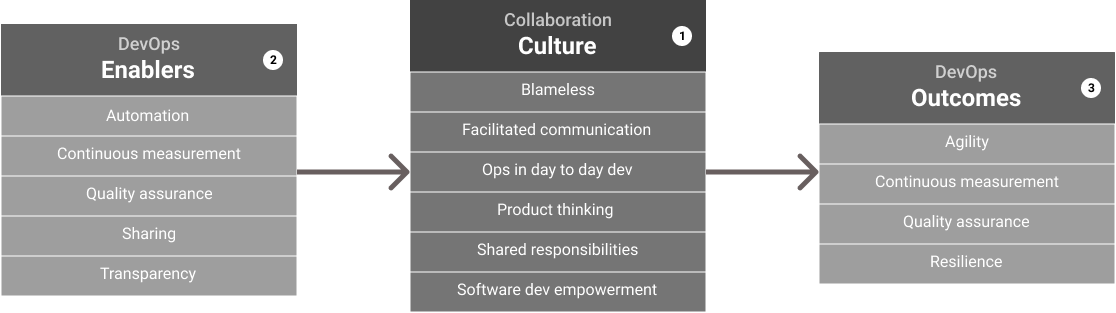
\includegraphics[width=.75\textwidth]{model.png}
  \caption{Categories and Relationships}
  \label{model}
\end{figure}

{
\color{blue}
Our proposed model has been applied to guide the DevOps adoption at the
Brazilian Federal Court of Accounts (TCU) where one of the authors of this study
works as a software developer. Bellow we present the details about the DevOps
adoption at TCU and explain the applicability and relevance of the model in a
practical scenario.
}
